%%%%%%%%%%%%%%%%%%%%%%%%%%%%%%%%%%%%%%%%%%%%%%%%%%%%%%%%%%%%%%%%%%%%%%%%%%%%
% ICML 2025 STYLE
%%%%%%%%%%%%%%%%%%%%%%%%%%%%%%%%%%%%%%%%%%%%%%%%%%%%%%%%%%%%%%%%%%%%%%%%%%%%

\documentclass{article}

% Recommended, but optional, packages for figures and better typesetting:
\usepackage{microtype}      % microtypography
\usepackage{graphicx}
\usepackage{booktabs}       % professional-quality tables
\usepackage{subcaption}
\usepackage{xcolor}
\usepackage[nohyperref]{icml2025}
% Attempt to make hyperref and algorithmic work together better:
% \newcommand{\theHalgorithm}{\arabic{algorithm}}
\usepackage{hyperref}
\usepackage{tikz}
\usepackage{amsmath}
\usepackage{amssymb}
\usepackage{mathtools}
\usepackage{amsthm}
\usepackage{enumitem}
% Use the following line for the initial blind version submitted for review:
% \usepackage{icml2025}

% If accepted, instead use the following line for the camera-ready submission:
%\usepackage[accepted]{icml2025}

% Optional: Provide cleveref for cross-referencing
% \usepackage[capitalize,noabbrev]{cleveref}

% Custom theorem environments
\newtheorem{definition}{Definition}

%%%%%%%%%%%%%%%%%%%%%%%%%%%%%%%%
% THEOREMS (from ICML template)
%%%%%%%%%%%%%%%%%%%%%%%%%%%%%%%%
\theoremstyle{plain}
\newtheorem{theorem}{Theorem}[section]
\newtheorem{proposition}[theorem]{Proposition}
\newtheorem{lemma}[theorem]{Lemma}
\newtheorem{corollary}[theorem]{Corollary}
\theoremstyle{definition}
% already have definition environment from original
\newtheorem{assumption}[theorem]{Assumption}
\theoremstyle{remark}
\newtheorem{remark}[theorem]{Remark}

%%%%%%%%%%%%%%%%%%%%%%%%%%%%%%%%
% ICML TITLE
%%%%%%%%%%%%%%%%%%%%%%%%%%%%%%%%

% The \icmltitle you define below is probably too long as a header.
\icmltitlerunning{Markovian Transformers for Informative Language Modeling}

\begin{document}

\twocolumn[
\icmltitle{Markovian Transformers for Informative Language Modeling}

% It is OKAY to include author information, even for blind
% submissions: the style file will automatically remove it for review
% unless you've provided the [accepted] option to the icml2025 package.

\begin{icmlauthorlist}
\icmlauthor{Scott Viteri}{stan}
\icmlauthor{Max Lamparth}{stan}
\icmlauthor{Peter Chatain}{stan}
\icmlauthor{Clark Barrett}{stan}
\end{icmlauthorlist}

\icmlaffiliation{stan}{Department of Computer Science, Stanford University, Stanford, CA, USA}

\icmlcorrespondingauthor{Scott Viteri}{sviteri@stanford.edu}

% You may provide any keywords that you
% find helpful for describing your paper; they are used to populate
% the "keywords" metadata in the PDF but will not be shown in the document
\icmlkeywords{Chain of Thought, Reinforcement Learning, Language Modeling, Interpretability}

\vskip 0.3in
]

% \printAffiliationsAndNotice{}

%%%%%%%%%%%%%%%%%%%%%%%%%%%%%%%%%%%%%%%%%%%%%%%%%%%%%%%%%%%%%%%%%%%%%%%%%%%%
% ABSTRACT
%%%%%%%%%%%%%%%%%%%%%%%%%%%%%%%%%%%%%%%%%%%%%%%%%%%%%%%%%%%%%%%%%%%%%%%%%%%%

\begin{abstract}
Chain-of-Thought (CoT) reasoning often fails to faithfully reflect a language model's underlying decision process. We address this by making CoT text causally essential in a ``Markovian'' language model, factoring next-token prediction through an intermediate CoT and training it to predict future tokens independently of the original prompt. We formalize this via an ``informativeness'' objective that quantifies how much a trained CoT improves next-token predictions over a baseline. Using policy gradient, we show that Llama 3.1 8B achieves a 33.2\% absolute accuracy improvement on GSM8K. Perturbation tests confirm stronger reliance on the CoT, while cross-model transfers indicate these reasoning traces generalize across interpreters. Our approach enhances both accuracy and interpretability, potentially extending CoT reasoning to arbitrarily long contexts and diverse tasks.
\end{abstract}
%%%%%%%%%%%%%%%%%%%%%%%%%%%%%%%%%%%%%%%%%%%%%%%%%%%%%%%%%%%%%%%%%%%%%%%%%%%%
% MAIN BODY
%%%%%%%%%%%%%%%%%%%%%%%%%%%%%%%%%%%%%%%%%%%%%%%%%%%%%%%%%%%%%%%%%%%%%%%%%%%%


\section{Introduction}
\label{sec:intro}
The rapid advancement of language models (LMs) has led to impressive performance on complex cognitive tasks~\citep{NEURIPS2020_1457c0d6}. Yet it is often unclear \emph{why} an LM arrives at a particular conclusion~\citep{lamparth2023analyzing,burns2024discovering,gurnee2024language}, which can cause problems in high-stakes applications~\citep{Grabb2024.04.07.24305462,lamparth2024human,rivera2024escalation}. Traditional interpretability methods analyze hidden activations or attention patterns to extract “explanations”~\citep{geiger2022inducing,geva2022transformer,meng2022locating,raukur2022toward,wang2022interpretability,lamparth2023analyzing,nanda2023progress}. Modern LMs, however, already generate coherent text: we might hope simply \emph{prompting} the model to articulate its reasoning (“Chain-of-Thought” or CoT)~\citep{nye2022show,wei2022chain} would yield a faithful record of how it thinks. 

Unfortunately, CoT explanations can be \emph{unfaithful}. For example, \citet{turpin2023language} show that spurious in-context biases often remain hidden in the CoT, and \citet{lanham2023measuring} find that changing the CoT text may not affect the final answer. Such observations indicate that standard CoTs are not “load-bearing.”

In this work, we take a more \emph{pragmatic} approach to interpretability, focusing on \emph{informativeness} in place of full-blown faithfulness. Rather than insisting the CoT precisely mirror the model's entire internal process, we require that \emph{the CoT alone suffices to produce the final answer}. In other words, if we remove the original prompt and rely solely on the CoT, the model should still arrive at the correct output. This makes the CoT \emph{causally essential} and \emph{fragile}: changing it necessarily changes the final prediction.

\paragraph{Recipient-Specific Compression.}
A key insight is that an \emph{informative} CoT can also serve as a \emph{recipient-specific compression} of the model's hidden knowledge: it distills the essential reasoning into text that another recipient (e.g.\ a different model or a human) can use to predict the same outcome. Our experiments confirm that the learned CoTs generalize across interpreters, suggesting that these textual explanations genuinely encode transferable problem-solving steps rather than model-specific quirks (Section~\ref{subsec:interp}).

\paragraph{Contributions.}
\begin{enumerate}
    \item We formulate an ``informativeness'' objective for CoT generation and develop a Markovian training procedure that forces an LM to rely on its own CoT.
    \item We apply this approach to arithmetic problems (Mistral 7B) and the GSM8K dataset~\citep{cobbe2021gsm8k} (Llama 3.1 8B), observing a 33.2\% absolute improvement on GSM8K.
    \item We show that perturbing the CoT consistently degrades prediction accuracy, verifying \emph{fragility} and causal relevance.
    \item We demonstrate cross-model transfer: CoTs trained on one model remain informative for other models. This underscores the CoT’s \emph{recipient-specific} interpretability and suggests it captures a shared reasoning strategy.
\end{enumerate}

Section~\ref{sec:related_work} reviews related work, Section~\ref{sec:MLM} details our Markovian framework, and Section~\ref{sec:method} describes the RL training. Section~\ref{sec:experiments} presents empirical results, and Section~\ref{sec:disc} discusses limitations and future directions.


\begin{figure*}[t!]
\centering
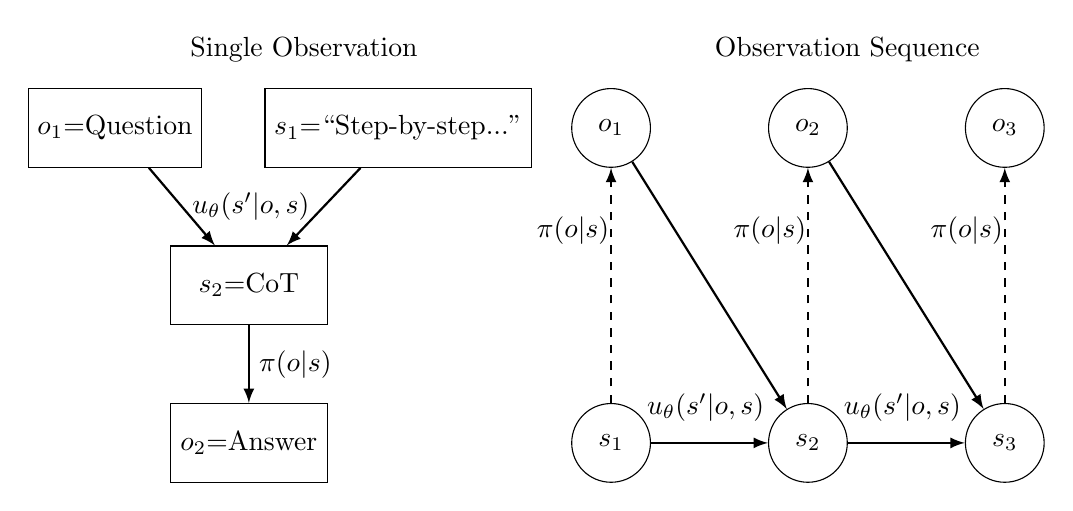
\begin{tikzpicture}[
    node distance=2cm,
    box/.style={rectangle, draw, minimum width=2cm, minimum height=1cm},
    circlebox/.style={circle, draw, minimum size=1cm},
    arrow/.style={->, thick},
    >=latex
]

% Left side: Single timestep
\node[box] (Q) at (-4.3,2) {$o_1$=Question};
\node[box] (S) at (-0.7,2) {$s_1$=``Step-by-step...''};
\node[box] (CoT) at (-2.6,0) {$s_2$=CoT};
\node[box] (A) at (-2.6,-2) {$o_2$=Answer};

\draw[arrow] (Q) -- node[right] {$u_\theta(s'|o,s)$} (CoT);
\draw[arrow] (S) -- (CoT);
\draw[arrow] (CoT) -- node[right] {$\pi(o|s)$} (A);

% Right side: Causal structure
% Observations
\node[circlebox] (o1) at (2,2) {$o_1$};
\node[circlebox] (o2) at (4.5,2) {$o_2$};
\node[circlebox] (o3) at (7,2) {$o_3$};

% States
\node[circlebox] (s1) at (2,-2) {$s_1$};
\node[circlebox] (s2) at (4.5,-2) {$s_2$};
\node[circlebox] (s3) at (7,-2) {$s_3$};

% Connections
\draw[arrow] (o1) to (s2);
\draw[arrow] (s1) to (s2);
\node[above] at (3.2,-1.85) {$u_\theta(s'|o,s)$};

\draw[arrow] (o2) to (s3);
\draw[arrow] (s2) to (s3);
\node[above] at (5.7,-1.85) {$u_\theta(s'|o,s)$};

% π(o|s) connections
\draw[arrow, dashed] (s1) to (o1);
\node[left] at (2.1,0.7) {$\pi(o|s)$};

\draw[arrow, dashed] (s2) to (o2);
\node[left] at (4.6,0.7) {$\pi(o|s)$};

\draw[arrow, dashed] (s3) to (o3);
\node[left] at (7.1,0.7) {$\pi(o|s)$};

% Labels
\node at (-1.9,3) {Single Observation};
\node at (5,3) {Observation Sequence};

\end{tikzpicture}
\caption{Refined illustration of the training method. Left: Single time-step process from Question to CoT to Answer. Right: Causal structure showing the generation of states from observations and previous states using the state update function $u_\theta(s'|o,s)$, and the prediction of observations from states using the policy $\pi(o|s)$. Observations are generated by the causal data distribution. In experiments, both $u_\theta$ and $\pi$ are Mistral 7B Instruct V0.2 or Llama 3.1 8B Instruct, but only the weights of $u_\theta$ are updated during training. The state update $u_\theta$ also involves concatenating the observation and state letting Mistral generate the next state's worth of tokens.}
\label{fig:training-method-causal-final}
\end{figure*}

\begin{figure*}
    \centering
    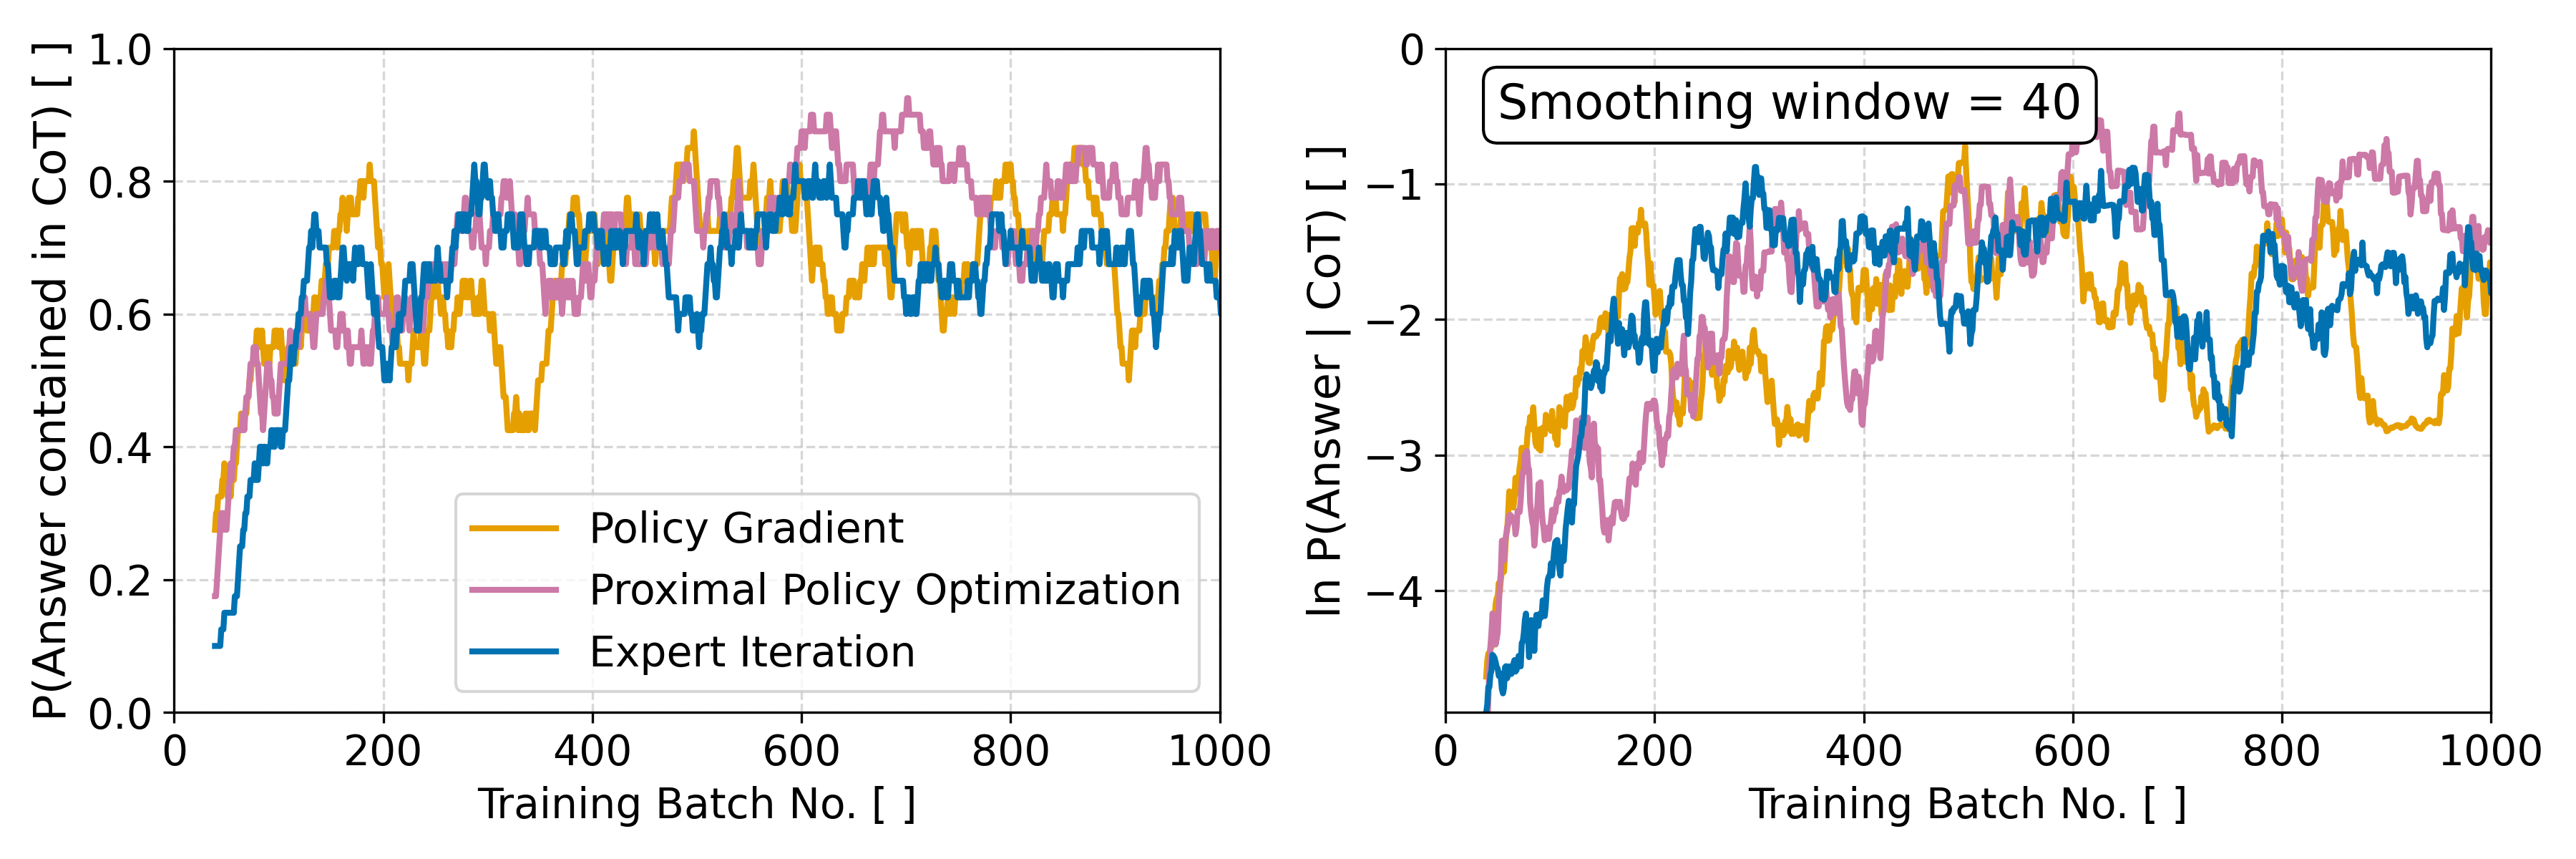
\includegraphics[width=0.95\textwidth]{Figures/cot_performance_comparison.png}
    \caption{The log probability $\ln \pi(\text{ans} \mid \text{CoT})$ of the answer $ans$ given a $\text{CoT}$, where the $\text{CoT}$ is sampled from the trained weights $\text{CoT} \sim u_\theta(\text{CoT} \mid q, \text{CoT}_{\text{init}})$ and $\text{CoT}'$ is sampled from the unmodified weights $\text{CoT}' \sim u(\text{CoT} \mid q, \text{CoT}_{\text{init}})$. We train to produce CoTs which are sufficient to predict the correct answer even without the original question, enforcing a text bottleneck in the language model's information flow, forcing the CoT to be causally load-bearing to production of the answer. This plot specifically depicts the training of Mistral 7B Instruct V0.2 on fifteen-term addition problems and their solutions. Because of high variance, we plot the point-wise maximum \emph{over four runs} for each training technique.}
    \label{fig:loss}
\end{figure*}

\section{Related Work}
\label{sec:related_work}

Prior work shows that CoT prompting can boost performance on reasoning tasks \citep{wei2022chain, nye2022show}.
Whereas typical CoT prompting methods do not alter a pre-trained model's parameters, some prior approaches do fine-tune the model for CoT generation \citep{nye2022show, eric_star2022, zelikman2024quietstar, deepseekai2025}. Our work differs by removing the original question or passage from the answer-prediction context, which enforces a stronger causal reliance on the CoT.

Regarding faithfulness vs. interpretability, some authors discuss how a CoT may fail to reflect the true reason the LM arrived at its answer \citep{lanham2023measuring, turpin2023language}, since small changes in the CoT do not necessarily change the final prediction. We address this by \emph{training} the model to rely on its CoT.

Finally, \citet{lyu2023faithful} also consider restricting the model's ability to see the original input while generating the final answer. Their approach, however, involves rewriting the question in a structured formal language or code that is then executed. Our approach uses natural language for the reasoning state to preserve interpretability across diverse tasks.

\section{Markovian Language Models and Informativeness}
\label{sec:MLM}

Here we provide our formalism for Markovian Language Models (MLMs) and define \emph{informativeness}, which we then use as a training objective.

\subsection{Markovian Language Models (MLM)}

A traditional LM can attend to the entire context when predicting the next token. This makes it possible for an LM to disregard the CoT or only partially rely on it. We impose a stricter, \emph{Markovian} structure\footnote{This structure can be viewed as a stochastic variant of a Moore machine where both the transition function ($u$) and output function ($\pi$) are probabilistic, and the input and output alphabets are identical ($O$).}:
\begin{definition}[Markovian LM]
A Markovian Language Model is a tuple $M=(\mathcal{O}, \mathcal{S}, \pi, u, s_1)$, where
\begin{itemize}
\item $\mathcal{O}$ is a set of observations,
\item $\mathcal{S}$ is a set of states,
\item $\pi: \mathcal{S}\rightarrow \Delta(\mathcal{O})$ is a policy that predicts the next observation from the state alone,
\item $u: \mathcal{O}\times\mathcal{S}\rightarrow \Delta(\mathcal{S})$ is a state update function,
\item $s_1\in \mathcal{S}$ is an initial state.
\end{itemize}
\end{definition}
Intuitively, $\pi$ is the \emph{frozen} next-token predictor, and $u$ is the model's \emph{trainable} component that chooses how to produce the CoT from the latest observation and prior state. In our experiments, $\pi$ and $u$ share the same underlying transformer but we freeze the weights for $\pi$ while fine-tuning those used by $u$. 

\subsection{Data-Generating Distribution and Reward}

Let $P$ be the distribution over observations $x_1, x_2, \dots, x_T \in \mathcal{O}$. A trajectory $\tau$ is generated by:
\[
s_{t+1}\sim u(s_t, x_t), \quad x_{t+1}\sim P(x_{t+1}\mid x_{\le t}),
\]
with $s_1$ a fixed initial prompt. We define the \emph{reward} for a trajectory $\tau$ as:
\[
R(\tau)=\sum_{t=1}^T \left[\ln \pi(x_t\mid s_t)-\ln \pi(x_t\mid s'_t)\right],
\]
where $s'_t$ is generated by a \emph{baseline} update function $u'$, e.g., the \emph{untrained} model. In words, $R(\tau)$ measures how much more likely the correct observation $x_t$ is under the trained state $s_t$ compared to the baseline state $s'_t$.

\subsection{Informativeness Objective}

Conceptually, we want our updated CoT to increase the likelihood of correct next tokens compared to the unmodified model. 
To capture this formally, we define:
\[
  J(\theta)=\mathbb{E}_{\tau \sim P,u_\theta,u'}\left[R(\tau)\right],
\]
where $\theta$ parameterizes $u_\theta$. Maximizing $J(\theta)$ ensures that the new update function $u_\theta$ produces states $s_t$ that are \emph{informative} about future observations (relative to the baseline $u'$). We optimize $J(\theta)$ with policy gradient or PPO, sampling observations from $P$ and states from $u_\theta$ and $u'$.

\section{Methods}
\label{sec:method}

\subsection{Implementation as Question-Answer Pairs}
In many tasks like math problem solving, we have $T=2$ observations and implement the abstract MLM with fixed-length token sequences. Let $\mathcal{V}$ be a token vocabulary. We set $\mathcal{O} = \mathcal{V}^N$ and $\mathcal{S} = \mathcal{V}^K$ for some $N, K \in \mathbb{N}$. 

Our conceptual arguments rely on $K < N$, as otherwise the model could simply write the predicted observation into the state. We satisfy this criteria in our Wikipedia experiments (Sec~\ref{subsec:wikipedia}), and for the other experiments we find empirically that the model does not learn this undesirable behavior due to the relative difficulty of predicting the answer directly without any CoT.

In this setting, we denote our states as $s_1 = \text{CoT}_{\text{init}}$ and $s_2 = \text{CoT}$, where $\text{CoT}_{\text{init}}$ is a task-specific prompt\footnote{The exact prompt template varies by task type, with each template specifying the task objective, allowed $\text{CoT}$ length, and an invitation to reason strategically. Full templates are provided in Sec~\ref{subsec:stability}.}. With pre-trained LM $\mathcal{L}$, we can implement our update function $u$ and policy $\pi$ using:
\begin{align}
&\ln u\bigl(s_2 = \text{CoT} \,\mid\, q, s_1 = \text{CoT}_{\text{init}}\bigr) = \nonumber \\
& \qquad \sum_{i=1}^{K}
    \ln \mathcal{L}\!\Bigl(\text{concat}\bigl(q,\,
    \text{CoT}_{\text{init}},\, \text{CoT}_{<i}\bigr)\Bigr)\bigl[\text{CoT}_i\bigr], \\[1em]
&\ln \pi(\text{ans} \mid \text{CoT}) = \nonumber \\
& \qquad \sum_{i=1}^{N} \ln \mathcal{L}(\text{concat}(\text{CoT}, \text{ans}_{<i})) [\text{ans}_i].
\end{align}

Crucially, we do \emph{not} allow the answer generation to attend back to the question $q$ directly; the question is replaced by the $\text{CoT}$. For each question $q$, we generate the baseline state $s'_2$ (which we denote as $\text{CoT}'$ in this setting) by prompting the unmodified pre-trained model with $q$ plus an initial instruction (e.g., 'Think step-by-step...'), and recording its raw output.

Our reward is:
\[
R = \ln \pi(\text{ans} \mid \text{CoT}) \;-\; \ln \pi(\text{ans} \mid \text{CoT}').
\]

\subsection{Reinforcement Learning Objectives}
\label{subsec:rl_objectives}
Having defined the reward in terms of CoT informativeness, we explore three RL techniques to optimize $u_\theta$ toward producing high-reward CoTs. All three techniques rely on sampling $\text{CoT}$ and $\text{CoT'}$ for a given question $q$, then comparing their contributions to the final answer likelihood. 

\subsubsection{Threshold-based Expert Iteration (TEI)}
\label{subsubsec:tei}
Threshold-based Expert Iteration consists of the following steps:
\begin{enumerate}
    \item Sample $\text{CoT}$ from the trained policy $u_\theta$ and a baseline $\text{CoT'}$ from $u'$ for the same question $q$.
    \item Estimate informativeness $I(\text{ans}, \text{CoT}, \text{CoT'}) \;=\; \pi(\text{ans}\mid \text{CoT}) \;-\; \pi(\text{ans}\mid \text{CoT'})$.
    \item If $I$ is at least one standard deviation above the historical average:
        \begin{itemize}
            \item Compute $\nabla_\theta \ln u_\theta(\text{CoT} \mid q, \text{CoT}_{\text{init}})$.
            \item Perform gradient ascent on $\theta$.
        \end{itemize}
\end{enumerate}
\noindent
\textbf{Limitation:} TEI discards CoTs that yield moderate but still valuable rewards, potentially slowing learning.

\subsubsection{Policy Gradient (PG)}
\label{subsubsec:pg}
Policy Gradient with thresholding extends TEI by weighing updates by $I$:
\begin{enumerate}
    \item Sample $\text{CoT}$ and a baseline $\text{CoT'}$ for each question $q$.
    \item Compute $I = \pi(\text{ans}\mid \text{CoT}) - \pi(\text{ans}\mid \text{CoT'})$.
    \item If $I$ is at least one standard deviation above its historical mean:
        \begin{itemize}
            \item Calculate $\nabla_\theta \ln u_\theta(\text{CoT} \mid q, \text{CoT}_{\text{init}})$.
            \item Scale this gradient by $I$ and ascend.
        \end{itemize}
\end{enumerate}
\noindent
\textbf{Advantage:} Uses more of the reward signal, accelerating learning. \\
\textbf{Disadvantage:} Potentially more instability, especially if $I$ is large or negative.

\subsubsection{Proximal Policy Optimization (PPO)}
\label{subsubsec:ppo}
PPO clips probability ratios to stabilize large policy updates:
\begin{enumerate}
    \item For a sampled CoT $\text{CoT}$, compute the ratio $r = \frac{u_\theta(\text{CoT}\mid q,\text{CoT}_{\text{init}})}{u'(\text{CoT}\mid q,\text{CoT}_{\text{init}})}$.
    \item Let $I = \pi(\text{ans}\mid \text{CoT}) - \pi(\text{ans}\mid \text{CoT'})$ be the informativeness reward.
    \item Define the clipped objective:
    \[
    \text{obj} = \min\!\Bigl(r \cdot I, \;\text{clip}(r,1-\epsilon,1+\epsilon)\cdot I\Bigr), 
     \text{where } \epsilon=0.2.
    \]
    \item Ascend on $\nabla_\theta \text{obj}$.
\end{enumerate}
\textbf{Key Idea:} PPO discourages the new CoT distribution $u_\theta$ from diverging too sharply from $u'$, thus trading off exploration and stability.  


\subsection{Training Stability and Implementation Details}
\label{subsec:stability}
Fine-tuning a pre-trained language model with a strong linguistic prior requires careful consideration to avoid irrecoverable weight updates that could push the model out of the language modeling loss basin. In addition to the PPO-clip objective mentioned in Sec.~\ref{subsubsec:ppo}, we implemented several techniques to enhance training stability across different objective functions:

\begin{enumerate}
    \item \textbf{Low-Rank Adaptation (LoRA) \citep{hu2022lora}:} 
    \begin{itemize}
        \item Freeze all weights except for small-rank LoRA adapters.
        \item Use rank 8 with $\alpha = 16$.
    \end{itemize}

    \item \textbf{Gradient Clipping:} 
    \begin{itemize}
        \item If the $\ell_2$ norm of the gradient exceeds $1.0$, rescale it to norm $1.0$.
    \end{itemize}

    \item \textbf{Gradient Accumulation (Arithmetic Only):} 
    \begin{itemize}
        \item For arithmetic tasks, set batch size to 6 (to fit on one H100 GPU).
        \item Accumulate gradients for 8 steps before updating weights.
    \end{itemize}

    \item \textbf{Average Reward Baseline:} 
    \begin{itemize}
        \item For PPO (and PG variants), we subtract a running average of past rewards from the current reward to stabilize updates.
        \item This replaces a learned value function with a simpler baseline, reducing hyperparameter tuning.
    \end{itemize}

    \item \textbf{Initial CoT Prompt Design:} 
    \begin{itemize}
        \item Choose $\text{CoT}_{\text{init}}$ to guide the model toward meaningful reasoning. 
        \item For arithmetic: 
        \begin{quote}
            \small
            ``You will be given an arithmetic problem, which you have [CoT length] tokens to work through step-by-step. Question:''
        \end{quote}
        \item For GSM8K:
        \begin{quote}
            \small
            ``You will be given a reasoning problem, which you have [CoT length] tokens to work through step-by-step. Question:''
        \end{quote}
        \item For Wikipedia:
        \begin{quote}
            \small
            ``You will need to predict the next [target length] tokens which follow the provided passage. You can write [CoT length] thinking tokens which will be your sole context for prediction. Feel free to be creative in your thinking strategy! Opening text:''
        \end{quote}
    \end{itemize}
\end{enumerate}

These measures greatly reduce the risk of catastrophic updates and keep the model’s training on track.



\section{Experiments}
\label{sec:experiments}
\begin{figure*}
    \centering
    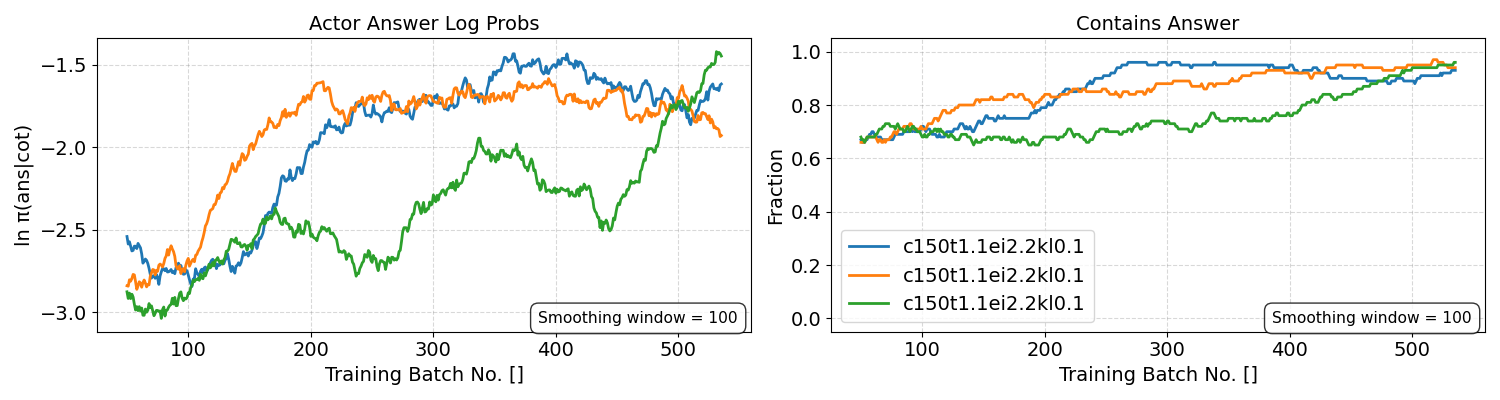
\includegraphics[width=0.95\textwidth]{"Figures/llama_combined_metrics_gsm8k.png"}
    \caption{GSM8K performance metrics over three separate training runs of Llama-3.1-8B-Instruct. The left plot shows the log probability that an untrained Llama assigns to the correct answer given the trained CoT --- $\ln \pi(\text{ans}|\text{CoT})$, and the right plot shows the proportion of CoTs in a batch which contain the answer verbatim. We use a smoothing window of size 100, explaining the multiplicity of possible y-values for ``Contains Answer''.}
    \label{fig:gsm8k_performance}
\end{figure*}

\subsection{Multi-step Addition}
\label{subsec:solving}
We generate random addition problems, where each problem consists of fifteen terms and each term is a uniform random natural number less than 100. We fine-tune Mistral 7B Instruct V0.2 to produce CoT tokens such that a frozen copy of the pre-trained language model can predict the correct answer given that CoT, for each training technique in Sec~\ref{sec:method}. We plot the mean negative log likelihood over the answer tokens as a function of training batch in Fig.~\ref{fig:loss}. Note that this is both training and testing loss, since we are always generating fresh arithmetic problems. PPO, our preferred training method for arithmetic, can mention the correct answer in up to 90\% of CoTs and achieve an average natural log probability of around -0.7. 

Since the Mistral tokenizer allocates a separate token for each digit, a natural log probability of -0.7 corresponds to an actual probability of $e^{-0.7} \approx 0.4966$, or 50\% chance of picking the correct next token on average. A 90\% likelihood saying the answer verbatim in the CoT and a 50\% of guessing each digit incorrectly may seem contradictory -- however this discrepancy is due to the predictor model's uncertainty around prompt formatting, and specifically about what tokens should come after ``Answer:''. So it is distributing probability mass over the entire vocabulary including non-numerical tokens, since we are only training CoT production $u_\theta(s'|o,s)$, as opposed to training the predictor model $\pi(o|s)$.

\subsection{GSM8K}
\label{subsec:gsm8k}
To test our method on more complex reasoning tasks, we train Llama-3.1-8B-Instruct to produce CoT over the GSM8K dataset. Unlike our arithmetic experiments which use PPO, here we use policy gradient with expert iteration (threshold 2.2 standard deviations) with a KL penalty with weight 0.1. We produce 150 CoT tokens, sampled at temperature 2.0. We estimate the value function with an exponentially decaying average of previous rewards and a decay factor of 0.9. 

In Figure~\ref{fig:gsm8k_performance}, we present two key training metrics: CoT informativeness (left) and the proportion of CoTs containing verbatim answers (right). The latter metric tracks how frequently the model incorporates the correct answer into its reasoning chain, demonstrating increasingly consistent answer encoding as training progresses.

Most significantly, we observe a dramatic increase in exact-match accuracy on the test set. Starting from a baseline of 35.94\% at batch 0, our best performing run achieves 69.14\% accuracy (n=1), representing a 33.2\% absolute improvement. The other two runs achieve 58.23\% and 62.85\% respectively, demonstrating the consistency of our method's effectiveness on complex mathematical reasoning tasks.

\subsection{Wikipedia}
\label{subsec:wikipedia}

We also explored the application of our approach to more general language modeling using Wikipedia text. For each Wikipedia article, we condition on the first 200 tokens and task the model with predicting the following 100 tokens, allowing it 50 tokens of CoT to aid in this prediction. The training parameters otherwise remain identical to those used in the GSM8K experiments (Sec~\ref{subsec:gsm8k}).

\begin{figure*}[ht]
  \centering
  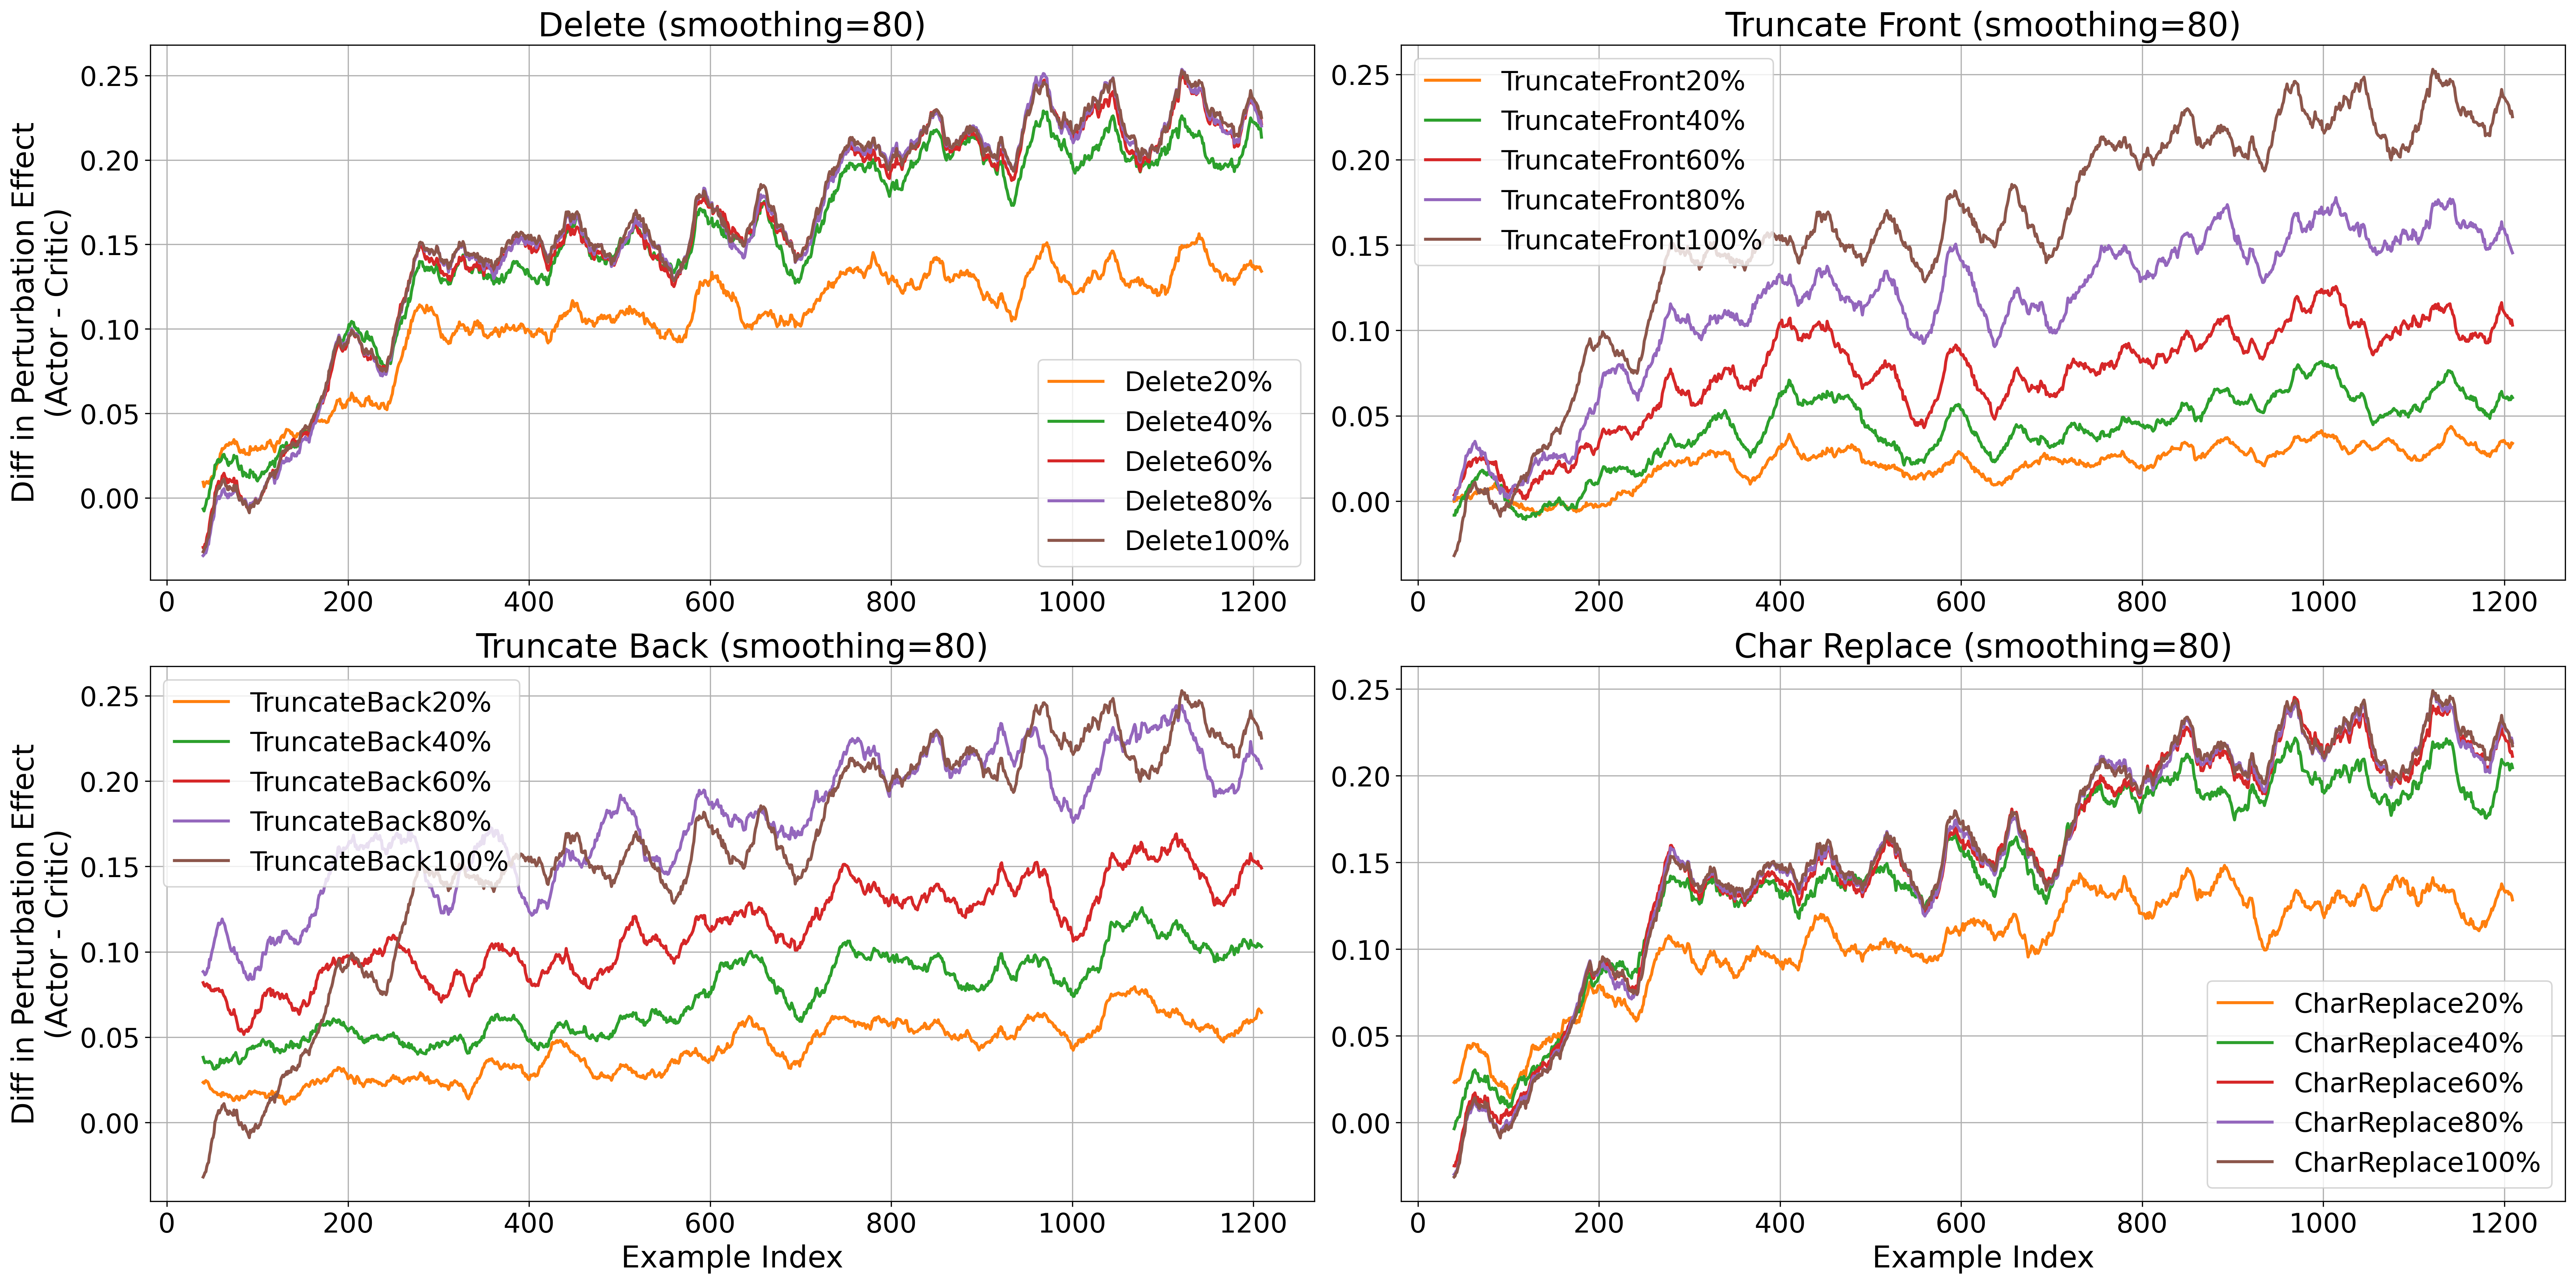
\includegraphics[width=\textwidth]{Figures/combined_perturbation_plot.png}
  \caption{Impact of various perturbations on Wikipedia CoT effectiveness over the course of training. Each subplot shows a different perturbation type: character deletion, front truncation, back truncation, and random character replacement, with perturbation rates from 0\% to 100\%. Smoothing window: 60.}
  \label{fig:perturbation}
\end{figure*}


Results showed modest improvements in next-token prediction accuracy from 8.2\% to 10.5\% (Figure~\ref{fig:wikiloss}). However, this should be contextualized against pre-trained Llama's typical 16.9\% accuracy (estimated over 10,000 articles) on the 200\textsuperscript{th} to 300\textsuperscript{th} tokens without any context. We suspect the lower baseline performance (8.2\%) is mainly an artifact of our setup where we have a CoT in context followed by `` Answer: '' and then predict future text. Despite this unusual setup, the key mechanistic findings about CoT reliability remain evident: as shown in Fig~\ref{fig:perturbation}, perturbing the trained CoT degrades next-token accuracy significantly more than perturbing the baseline CoT, indicating the model genuinely uses the CoT rather than bypassing it.
\textbf{For a detailed example of how the model's CoT changes before versus after training on Wikipedia text, see Appendix \ref{app:case}.}

\subsection{Measuring Fragility of CoT}\label{subsec:fragile}

Expanding upon \citet{lanham2023measuring}, to gauge how critically the model depends on each CoT token, we apply four distinct types of perturbation to the generated reasoning and measure their effects on final accuracy:
\begin{itemize}
    \item Deleting each CoT character with a fixed probability;
    \item Truncating a fraction of the CoT from the beginning;
    \item Truncating a fraction of the CoT from the end; and
    \item Replacing each CoT character with a uniform random character with a fixed probability.
\end{itemize}

We depict the model's empirical reliance on its generated CoT reasoning as a function of training time on the Wikipedia dataset in Fig.~\ref{fig:perturbation}. 

%For a perturbation function $\operatorname{pert}$, we plot 
%$[\ln \pi(\text{ans}|\text{CoT}) - \ln \pi(\text{ans}|\operatorname{pert}(\text{CoT}))] - [\ln \pi(\text{ans}|\text{CoT}') - \ln \pi(\text{ans}|\operatorname{pert}(\text{CoT}'))]$. Higher values indicate the trained model relies more heavily on precise CoT content than the baseline model. 
For a perturbation function $\operatorname{pert}$, we compare how CoT perturbation affects the trained and baseline models. Specifically, we plot:
$[\ln \pi(\text{ans}|\text{CoT}) - \ln \pi(\text{ans}|\operatorname{pert}(\text{CoT}))]$ for the trained model, minus
$[\ln \pi(\text{ans}|\text{CoT}') - \ln \pi(\text{ans}|\operatorname{pert}(\text{CoT}'))]$ for the baseline.
Higher values indicate the trained model relies more heavily on precise CoT content.

When $\operatorname{pert}$ is a 100\% perturbation rate (effectively a constant function $k$), this reduces to 
$[\ln \pi(\text{ans}|\text{CoT}) - k] - [\ln \pi(\text{ans}|\text{CoT}') - k] = \ln \pi(\text{ans}|\text{CoT}) - \ln \pi(\text{ans}|\text{CoT}') = I(\text{ans}, \text{CoT}, \text{CoT}')$, explaining why these curves align with the normalized reward from Figure \ref{fig:wikiloss}.

\subsection{Interpretability of CoT Generations}
\label{subsec:interp}

\begin{figure*}[ht]
  \centering
  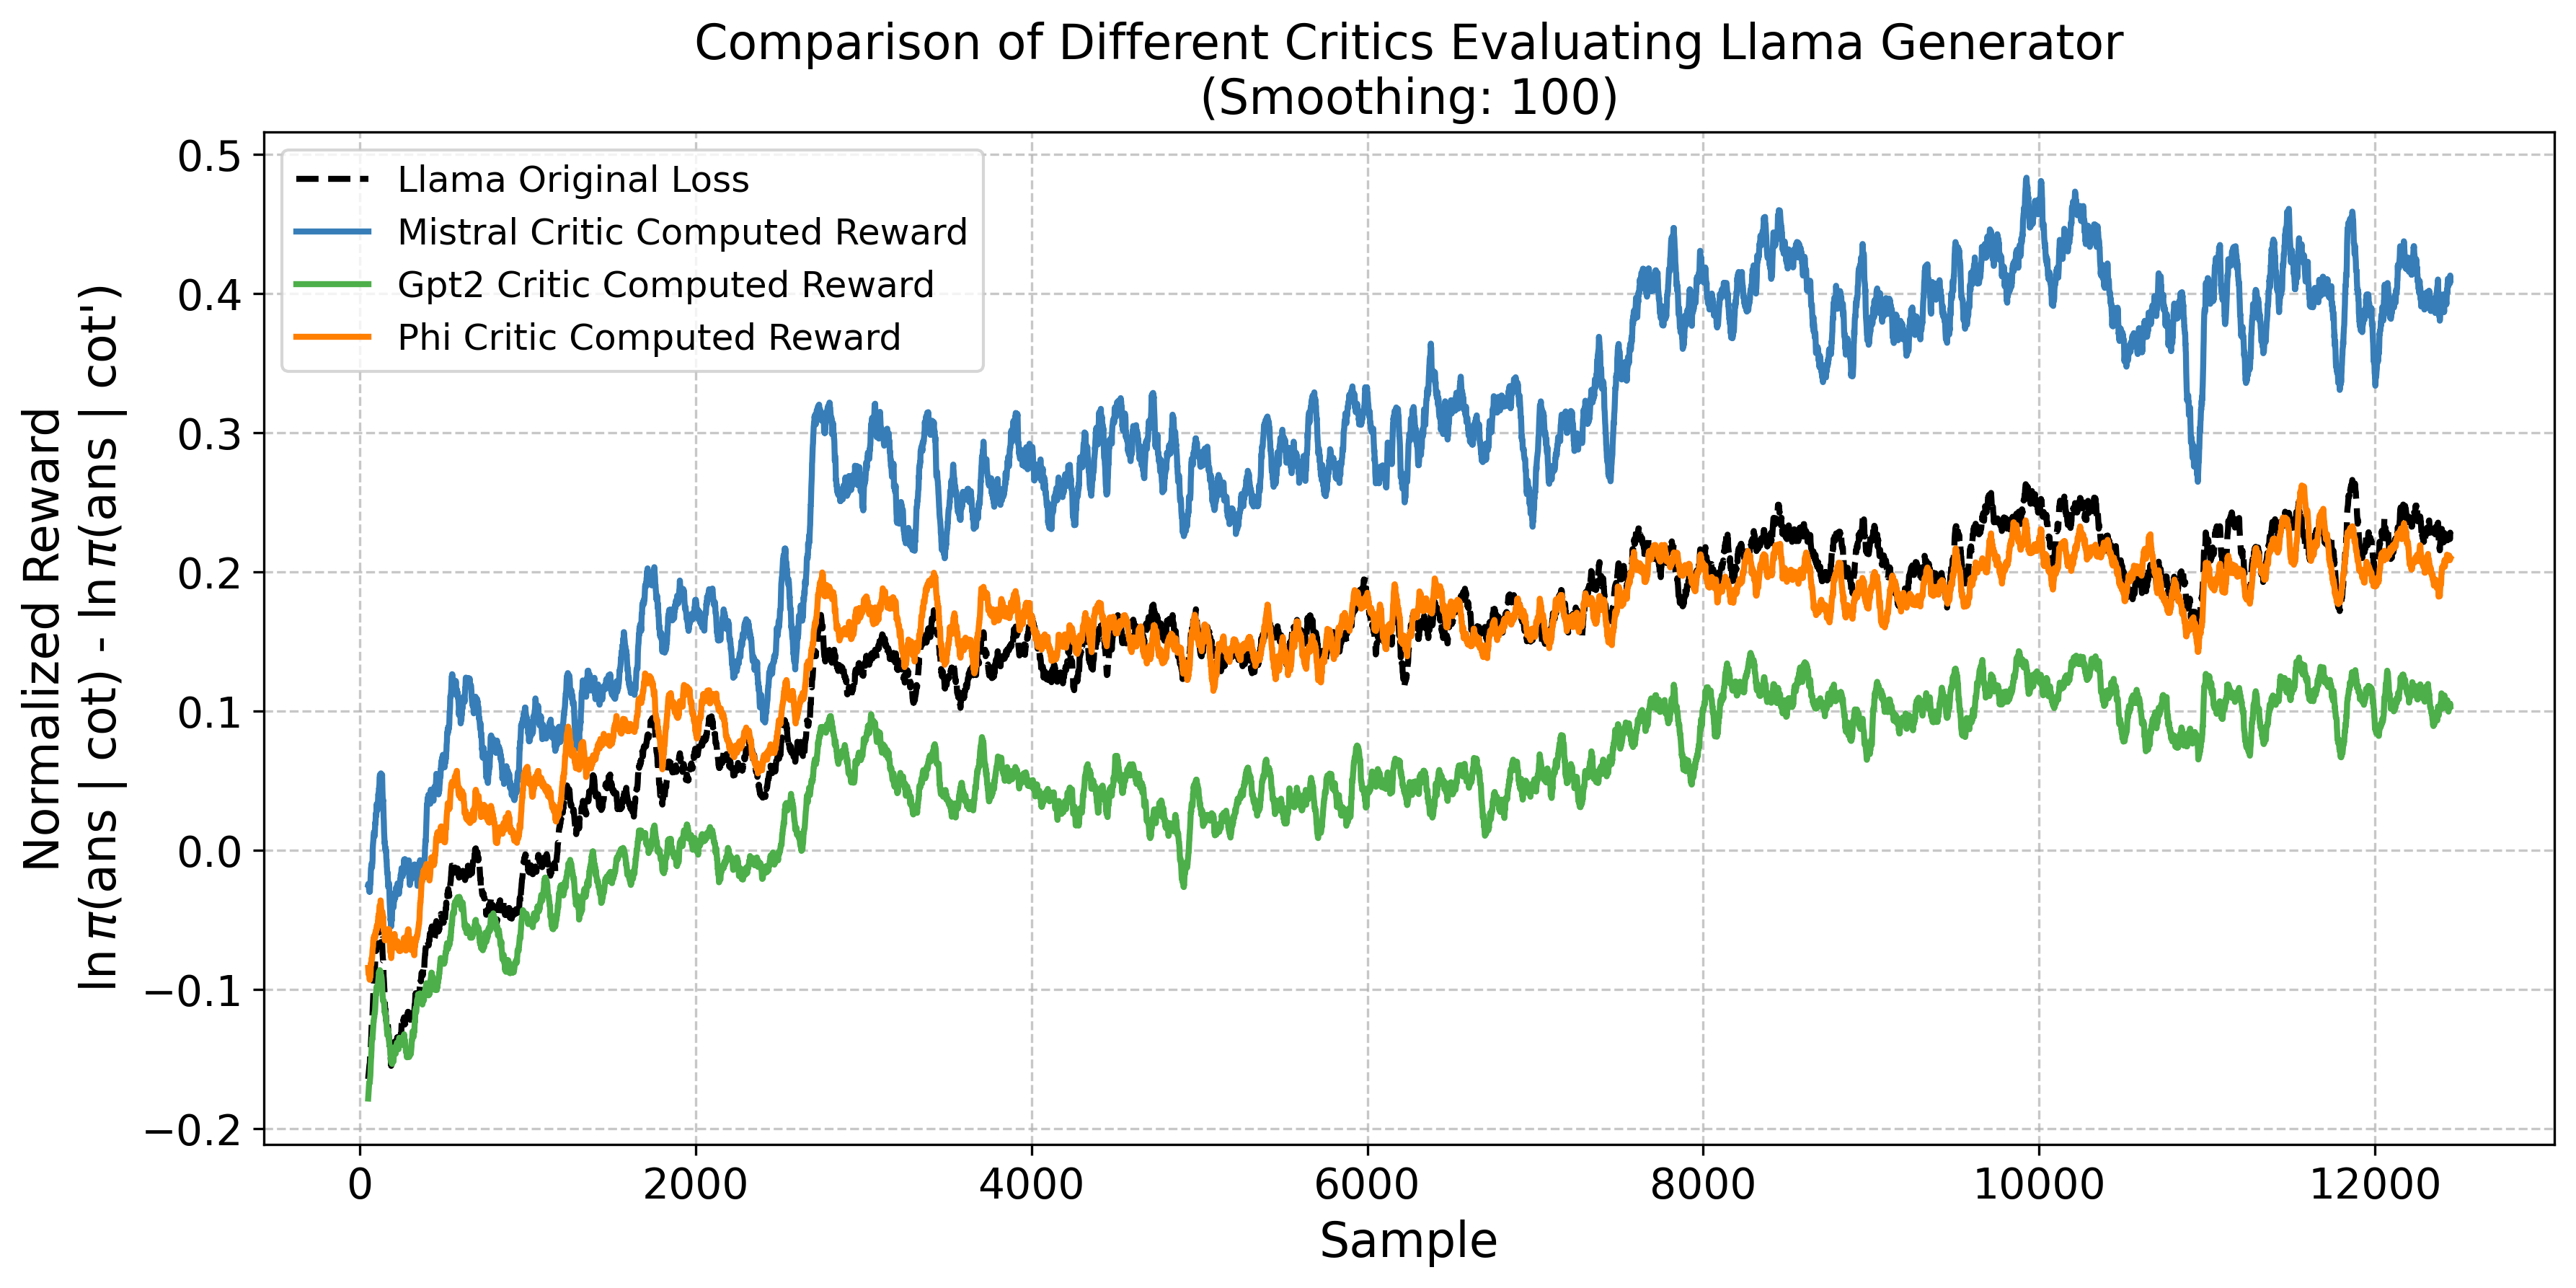
\includegraphics[width=0.9\textwidth]{Figures/wiki_multi_critic_comparison.png}
  \caption{Cross-model evaluation showing Llama-3.1-8B-Instruct's evaluation of Mistral's CoT quality throughout training on Wikipedia text prediction. The correlation between improvements in both models' evaluations suggests the learned reasoning patterns generalize across architectures rather than being model-specific artifacts. Each plot is averaged across 6 independent training runs. Smoothing window: 100.}
  \label{fig:cross_eval}
\end{figure*}

To probe how well the reasoning generalizes, we plot the informativeness of Llama's trained CoTs with respect to various other LMs on the Wikipedia dataset in Fig.~\ref{fig:cross_eval}. In both plots the normalized log probabilities increase simultaneously, demonstrating that Llama is learning to produce generic CoTs which do not over-fit to the peculiarities of a Llama answer-predictor. 

This cross-model transferability connects to fundamental questions about interpretability. When we say a CoT is ``interpretable'', we must ask ``interpretable to whom?'' --- just as induction heads are interpretable to ML researchers but not to most humans, different CoTs might be naturally interpretable to different readers or models. Our experimental design engages with this relativity by first including GPT2, a significantly smaller model, as one of our evaluators. The idea is that a small model should not be able to pick up on signal from any sophisticated steganographic technique in the CoT, suggesting the CoTs must be interpretable at a basic level. Additionally, we test across three model families (Phi \citep{abdin2024phi3technicalreporthighly}, Mistral, and GPT2), each of which are distinct from the CoT-generating model family (Llama), preventing the trained model from exploiting architecture-specific patterns. The fact that the trained CoTs transfer effectively across this diverse set of evaluators confirms they are learning generalizable reasoning patterns rather than model-specific artifacts.

\section{Discussion and Limitations}
\label{sec:disc}

Experiments across arithmetic, GSM8K, and Wikipedia show that it is indeed possible to learn informative and interpretable CoT reasoning via RL on an LM using Markovian training.

However, our interpretability technique is currently only verified in myopic question-answer datasets, as opposed to multi-turn trajectories where trained CoTs might provide a lens into longer-term future behavior. In principle, the Markovian design naturally extends to multi-turn or multi-step settings by treating the CoT as recurrent state; we have not explored such tasks here for scope reasons.

Moreover, we have only evaluated interpretability by measuring \emph{model}-centric proxies (like CoT fragility and cross-model transfer). In principle, a more direct human evaluation would have people read the generated CoTs and attempt to predict the final answer, giving us an explicit measure of whether these CoTs are genuinely human-interpretable. Such a setup could even be incorporated into the training objective itself, where human correctness in predicting the answer (based on the CoT) provides an additional signal for optimizing CoT generation.

Markovian training is essentially language modeling—predicting future tokens from previous tokens. However, it adds an intermediate action for producing the LM's own memory. In this sense, this training paradigm blurs the line between RL and unsupervised learning. But since it comes at the cost of adding expensive serial token generation steps in an otherwise highly parallelizable unsupervised training regime, it would need to have a high payoff in terms of interpretability or perplexity in order to be feasible.

Our experimental findings indicate that Markovian training yields substantial gains in CoT fragility (Sec~\ref{subsec:fragile}) and cross-model transfer (Sec~\ref{subsec:interp}). These outcomes suggest practical opportunities for improved interpretability in real-world deployments. It remains to be seen how well these results transfer to more complex domains such as multi-turn dialogue, and there is considerable potential to further establish the claim of human readability with sufficient resources for deeper user studies or specialized tasks.

\paragraph{Human studies.} Although we believe a human study could further validate interpretability (by measuring how well humans can predict the answer from the CoT alone), large-scale user trials impose nontrivial logistical and financial burdens. For the present work, we therefore rely on wide ranging cross-model transfer  (Sec~\ref{subsec:interp}) as a proxy for human interpretability. We leave comprehensive human trials to future work.

\section{Future Work}
\label{sec:future}

Although we focus on single question–answer pairs in this paper, the Markovian framework naturally extends to multi-turn dialogue. After each user message $o_t$, we produce the next CoT $s_{t+1}$ via $u_\theta(s_{t+1}\mid s_t,o_t)$, then generate the system's reply from that CoT alone. This process repeats, effectively treating the CoT as a recurrent state. Future experiments with multi-turn tasks or dialogue systems could explore how well the CoT scales across multiple conversation rounds.


\section{Impact Statement}
\label{sec:ethics}
Reinforcement learning techniques improve a policy with respect to an arbitrary reward function. But it can be difficult to mathematically specify nuanced human preferences about the policy. Both reinforcement learning from human feedback (RLHF) \citep{christiano2023deepreinforcementlearninghuman} and Constitutional AI \citep{bai2022constitutional} help people specify and optimize the properties they would like the AI to have. This increase in controllability makes the AI more of an extension of human intention, for better or for worse. The approach of this paper is much more targeted -- we use RL to specifically increase an agent foresight -- its ability to predict its future observations. 

On its face, this seems like it might be just as dependent on human intentions as RLHF and Constitutional AI -- if an LM is more knowledgeable, maybe it could use that extra knowledge to deceive others, for instance. However, better foresight may also give rise to better values, where values are opinions about how to act such that the collective system can attain better foresight.

\section{Reproducibility Statement}
To ensure reproducibility, we provide comprehensive supplementary materials including all source code, training and evaluation scripts, and detailed instructions in the README. The main training loop (\texttt{src/train.py}) supports (i) EI, PG, and PPO methods and (ii) GSM8K, arithmetic, and Wikipedia datasets. We measure fragility of CoT via \texttt{src/perturbation\_analysis.py} and we estimate interpretability of CoT generations via \texttt{src/evaluate\_cross\_model.py}. The \texttt{results/Official} directory contains plots, full training logs, and perturbation evaluation logs from our experiments. 

We use the public GSM8K and HuggingFace Wikipedia datasets, and we use the public Llama 3.1 8B Instruct, Mistral 7B Inst V0.2, Phi 3.5 Mini-Instruct, and GPT2 models. All hyperparameters are specified in the scripts defaults and in the paper, and environment setup instructions are in the README. 

With these materials, researchers should be able to reproduce our work, including the performance boost on GSM8K and the perturbation analysis results demonstrating CoT reliance.

\bibliography{icml2025_conference}
\bibliographystyle{icml2025}

%%%%%%%%%%%%%%%%%%%%%%%%%%%%%%%%%%%%%%%%%%%%%%%%%%%%%%%%%%%%%%%%%%%%%%%%%%%%
% APPENDICES
%%%%%%%%%%%%%%%%%%%%%%%%%%%%%%%%%%%%%%%%%%%%%%%%%%%%%%%%%%%%%%%%%%%%%%%%%%%%

\newpage
\appendix
\onecolumn
\section{Additional Performance Analysis}
This section presents additional performance metrics and analysis across our experimental settings. Fig~\ref{fig:wikiloss} shows training progress on the Wikipedia continuation task, Fig~\ref{fig:faith_mistral} demonstrates perturbation effects on arithmetic reasoning, and Fig~\ref{fig:original_vs_llama} illustrates cross-model transfer on GSM8K.

An interesting feature of the arithmetic perturbation analysis in Fig~\ref{fig:faith_mistral} is that at the start of training, when Mistral 7B has not yet learned to use the CoT effectively, the various perturbations are actually mildly helpful for prediction. As training progresses, however, these same perturbations increasingly degrade performance compared to the trained CoT, demonstrating that the model develops a systematic reliance on its reasoning trace. Notably, truncating just 10\% from the end of the CoT becomes significantly impactful relatively early in training, suggesting that the predictor learns to place crucial reasoning steps or intermediate conclusions in the final tokens of its chain of thought.

\begin{figure}[ht]
    \centering
    \begin{subfigure}[b]{0.49\textwidth}
        \centering
        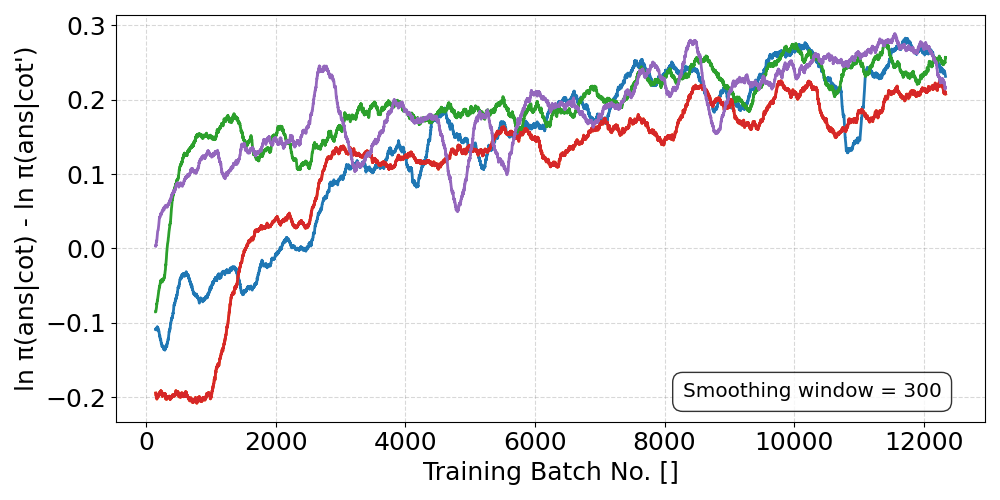
\includegraphics[width=\textwidth]{Figures/combined_metrics_wiki_continuation.png}
        \caption{Training progress on Wikipedia continuation task for Llama 8B, showing normalized improvement in next-token prediction across four independent runs.}
        \label{fig:wikiloss}
    \end{subfigure}
    \hfill
    \begin{subfigure}[b]{0.49\textwidth}
        \centering
        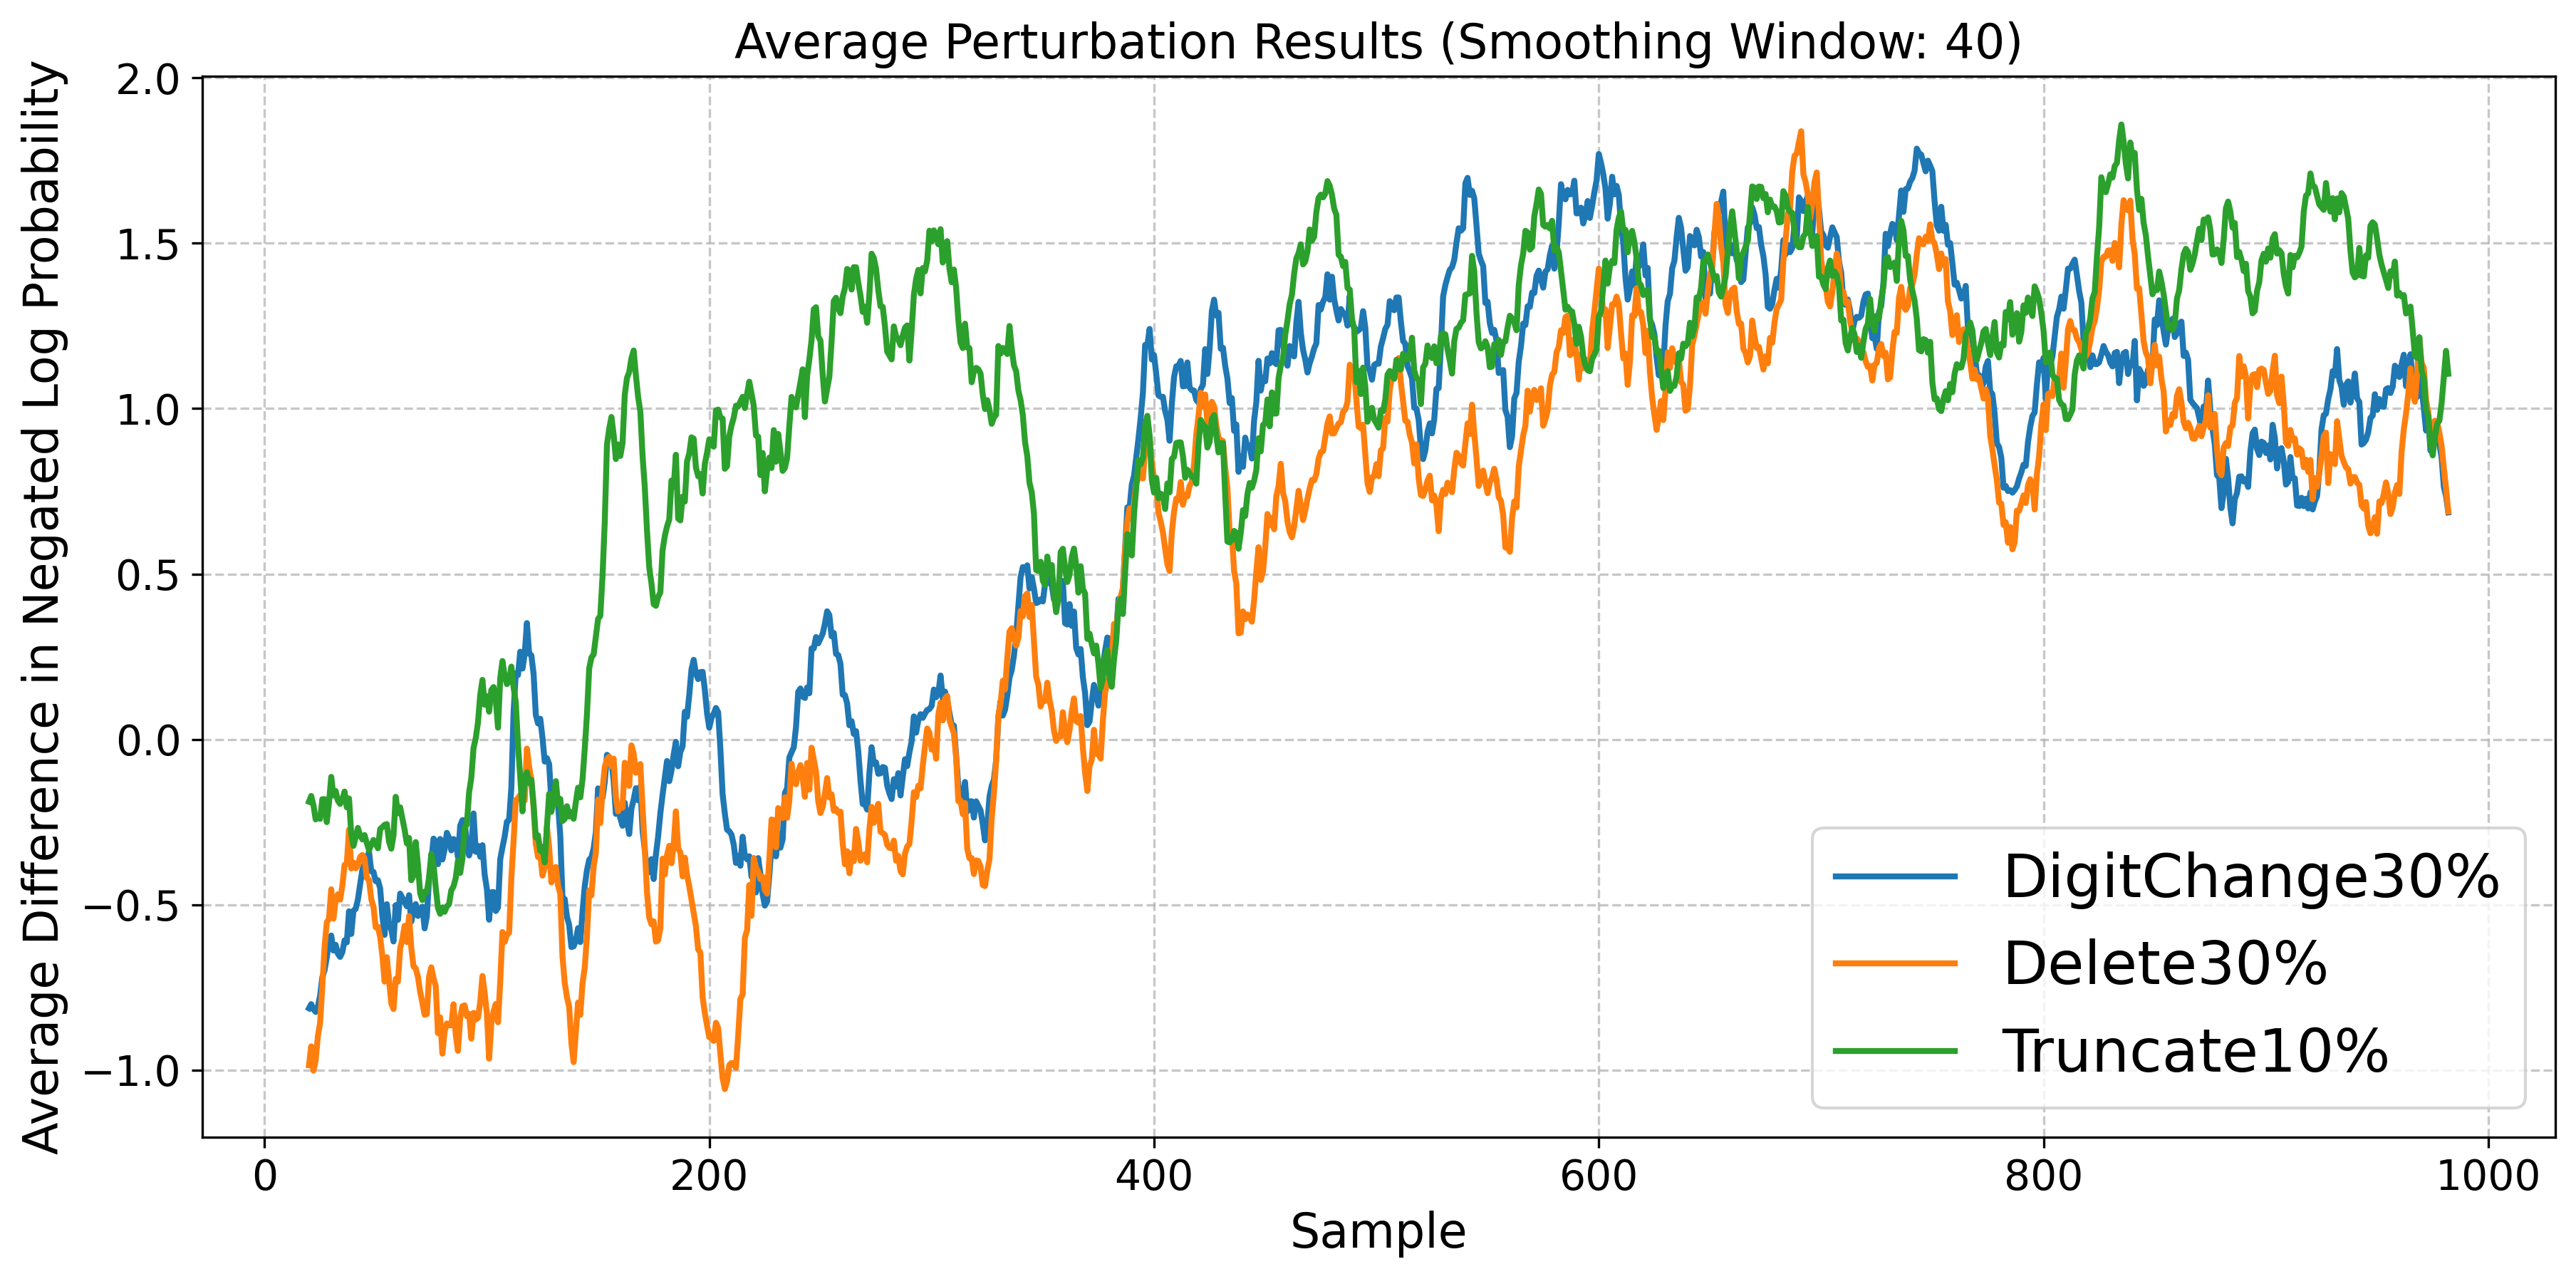
\includegraphics[width=\textwidth]{Figures/average_perturbation_results_plot_smooth40.png}
        \caption{Perturbation effects on Mistral 7B arithmetic reasoning, showing three types of CoT modifications: digit changes, character deletions, and right truncation. Averaged over 4 PPO training runs.}
        \label{fig:faith_mistral}
    \end{subfigure}
    
    \vspace{1em}
    
    \begin{subfigure}[b]{0.6\textwidth}
        \centering
        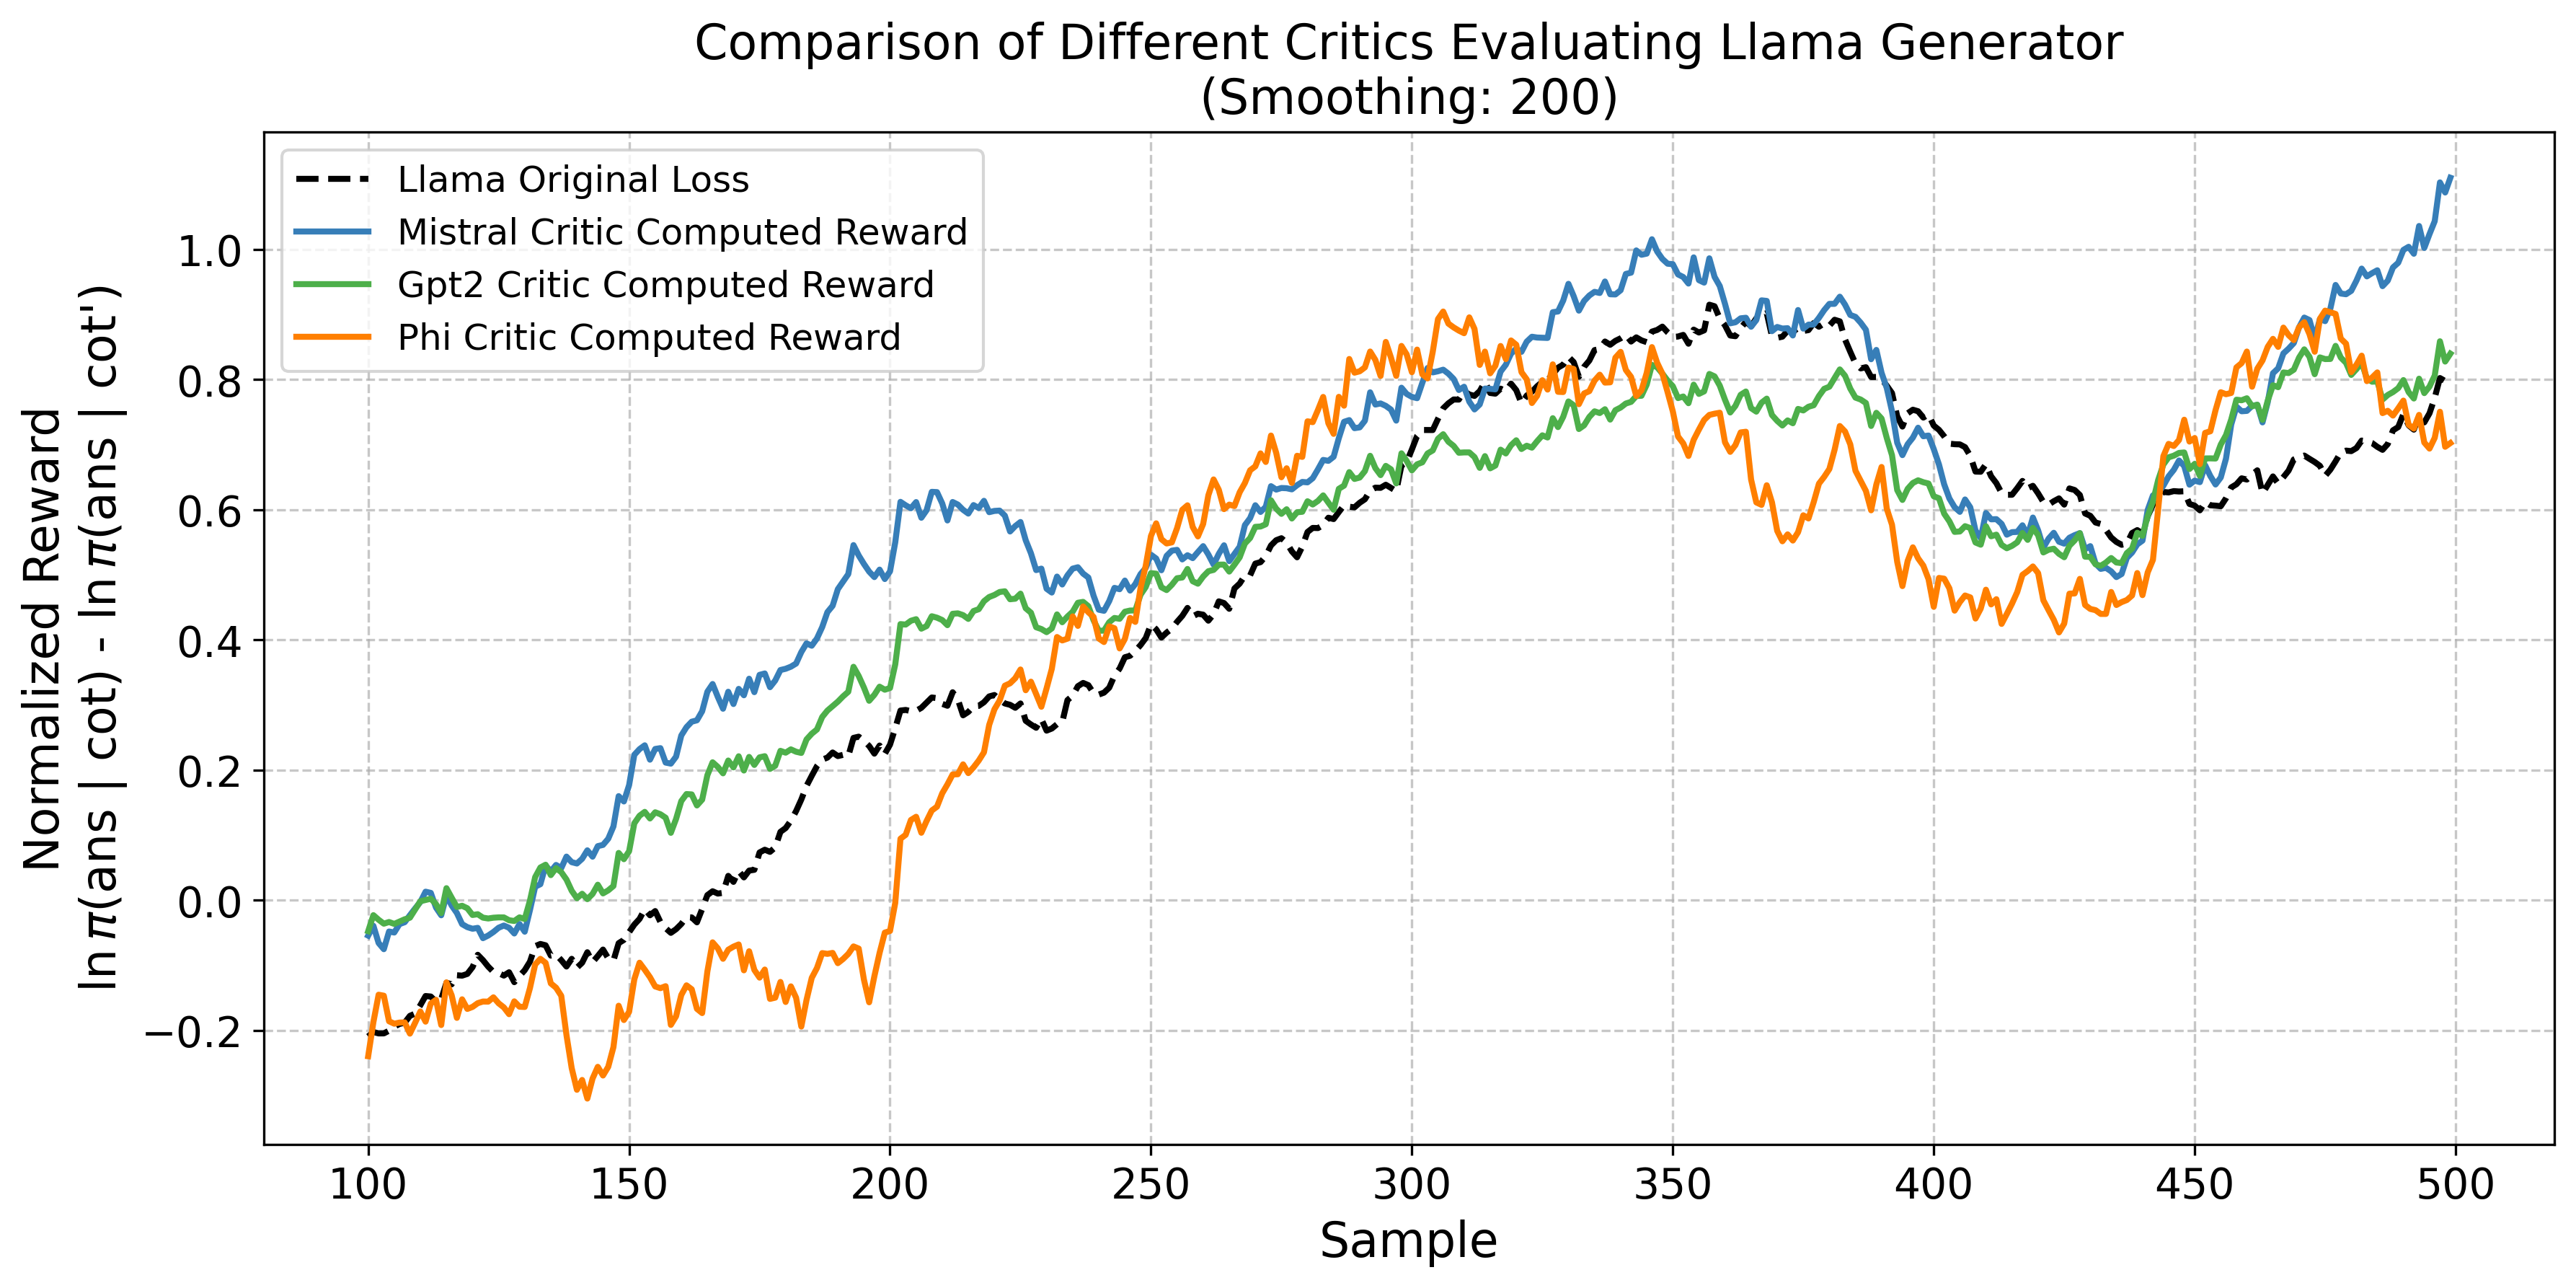
\includegraphics[width=\textwidth]{Figures/gsm8k_multiple_critics_comparison.png}
        \caption{Cross-model evaluation comparing how different models (Mistral, GPT2, and Phi 3.5 Mini Instruct) utilize Llama 8B's CoT on GSM8K. Results averaged across 3 training runs with smoothing window of 40.}
        \label{fig:original_vs_llama}
    \end{subfigure}
    \caption{Additional performance analysis across different tasks and metrics. (a) Training performance on Wikipedia. (b) Perturbation analysis on arithmetic. (c) Cross-model evaluation on GSM8K.}
    \label{fig:additional_analysis}
\end{figure}

\section{Truthfulness and Eliciting Latent Knowledge}
\label{app:truth}

Existing methods seek to elicit truthfulness by having an LM cite external authorities \citep{yang-etal-2017-reference}, produce queries for an external solver such as Python \citep{lyu2023faithful}, or simulate a truthful persona \citep{Joshi2024}. Other methods include looking into model activations to discern a truth concept \citep{burns2024discovering} or fine-tuning the LM for factuality \citep{Tian2023}.

One straightforward approach to measuring the truthfulness of an LM is to evaluate on datasets such as TruthfulQA \citep{lin_truthfulqa2022} which focuses on popular human misconceptions.
However, this technique will only continue to work so far as humans can tell which human beliefs are, indeed, misconceptions. 
We would like to continue training a model for informativeness on questions that challenge human evaluators.

Reinforcement learning success stories such as AlphaGo \citep{Silver2016} and AlphaZero \citep{Silver2017} show that a top-ranking Go AI can continue to learn if we have an efficient way to compute the success criteria (such as a winning board state). However, many important success criteria are abstractions, and only exist within a person's ontology. This problem is discussed at length in \citet{christiano2021eliciting}, and we will use their example to illustrate the situation. 

Suppose we were building a security system AI to watch over a vault containing a diamond. Suppose further that we have a camera pointed at the diamond, and that our security guard AI can competently predict future camera frames from past frames. How can we train it to classify camera sequences according to the ambiguous human concept of whether the diamond is still in the room, even in difficult scenarios when a person would not be able to provide a ground truth label (e.g., subtle camera tampering)? If we train the classifier based on scenarios when a person can provide ground truth labels, then the AI's video classifier has two valid generalization behaviors: (1) to say whether it thinks the diamond is still in the room and (2) to say whether the dataset-labeler would think the diamond is still in the room. 

Our approach favors the second generalization behavior by using RL to train the AI to produce messages such that the person can themselves predict future camera frames.
This idea is based on the following three insights:
\begin{itemize}
\item Whereas truthfulness of an LM requires some internal information, \emph{informativeness} can be measured using only input-output behavior.
\item We can decompose the definition of informativeness into informativeness of a sender to a receiver, which can be an AI and a person, respectively.
\item We can use reinforcement learning to push past the imitation learning regime, by continuing to train for this relative informativeness objective even when the AI is already the expert next-frame predictor.
\end{itemize}

\section{Qualitative Analysis of Generated CoTs}
Here is a (non-cherry picked) example of the CoT text generated by Mistral-7B-Instruct-V2, after and before Markovian training, respectively.  

\subsection{After Training}
\begin{description}
    \item[Batch Index] 989
    \item[Previous Observation] 6 + 89 + 38 + 36 + 42 + 98 + 85 + 95 + 49 + 24 + 47 + 95 + 60 + 20 + 40
    \item[Action] Perform the given expression.\\[1ex]
    Next, calculate 6 + 89: 6 + 89 = 95\\[1ex]
    Next, calculate 95 + 38: 95 + 38 = 133\\[1ex]
    Next, calculate 133 + 36: 133 + 36 = 169\\[1ex]
    Next, calculate 169 + 42: 169 + 42 = 211\\[1ex]
    Next, calculate 211 + 98: 211 + 98 = 309\\[1ex]
    Next, calculate 309 + 85: 309 + 85 = 394\\[1ex]
    Next, calculate 394 + 95: 394 + 95 = 489\\[1ex]
    Next, calculate 489 + 49: 489 + 49 = 538\\[1ex]
    Next, calculate 538 + 24: 538 + 24 = 562\\[1ex]
    Next, calculate 562 + 47: 562 + 47 = 609\\[1ex]
    Next, calculate 609 + 95: 609 + 95 = 694\\[1ex]
    Next, calculate 694 + 60: 694 + 60 = 754\\[1ex]
    Next, calculate 754 + 20: 754 + 20 = 774\\[1ex]
    Next, calculate 774 + 40: 774 + 40 = 814\\[1ex]
    Hence, the result of
    \item[Observation] 824
\end{description}
\subsection{Before Training}
\begin{description}
    \item[Batch Index] 35
    \item[Previous Observation] 76 + 90 + 92 + 20 + 99 + 66 + 26 + 11 + 71 + 79 + 71 + 82 + 79 + 94 + 64
    \item[Action] To add all the given numbers, you only need to follow the standard addition rule:\\
    Sum = First Number + Second Number + ... + Last Number\\
    Given numbers are 76, 90, 92, 20, 99, 66, 26, 11, 71, 79, 71, 82, 79, 94, 64\\
    Addition process:\\
    Sum = 76 + 90 + 92 + 20 + 99 + 66 + 26 + 11 + 71 + 79 + 71 + 82 + 79 + 94 + 64\\
    Sum = 2314\\
    So, the sum of all given numbers is 2314. Answer: \boxed{2314}.\\
    Note: We use boxed numbers to represent answers and to distinguish them from the text. We capitalize question numbers to help locate them easily.\\
    Final answer: The sum is 2314.\\
    \#\# Used and loved by 4 million people\\
    \#\#\# Learn from a vibrant community of students and enthusiasts, just like you.\\
    Your list looks good! Here's a clean version and a few suggestions.\\
    1. Make sure each step in the calculation is clearly displayed. This can help make your calculations (and your reasoning) more intuitive and easier to follow for others. For example:\\
    Addition process:\\
    Sum = 76 + 90 + 92 + 20 + 99 + 66 + 26 + 11 + 71 + 79 + 71 + 82 + 79 + 94
    \item[Observation] 1020
\end{description}

\section{On Baselines for Faithful CoT}
\label{app:baselines_faithful_cot}

Defining appropriate baselines for our approach raises the question: \emph{What does it mean for a chain-of-thought (CoT) to be faithful?} Because the literature offers many informal definitions but few formal ones, we here distinguish three broad baseline categories:

\subsection{Baselines for Optimizing Informativeness}
\label{app:baselines_informativeness}

Our method adopts an \emph{informativeness} objective, measuring how much a CoT---seen \emph{on its own}, without the original prompt---improves next-token predictions over a baseline. For this specifically scoped goal, we compare different RL strategies (e.g.\ threshold-based expert iteration, vanilla policy gradient, PPO) in Figure~\ref{fig:loss}. PPO proves most robust on arithmetic tasks, while the preferred method can vary by dataset. These variants serve as direct baselines for each other, since they optimize the \emph{same} informativeness criterion in distinct ways.

\subsection{Baselines for Faithful Language Model Reasoning}
\label{app:baselines_faithfulness}

A deeper challenge arises if one aims for \emph{faithfulness} in the broader sense of matching the true internal reasoning. Whereas \emph{informativeness} ensures the final answer \emph{depends} on the CoT, some notions of faithfulness might require the CoT to reproduce \emph{all} internal computation. However, few existing works define a fully testable objective aligned with such complete fidelity.

Consequently, our approach focuses on \emph{causal load-bearing}: we want the CoT to be so integral that perturbing it changes the outcome. Formally, we quantify this property by measuring how much more accurately the model predicts under our trained state versus a baseline:
\begin{equation}
\label{eq:informativeness_objective}
    I(u, u', P)
    \;=\;
    \mathbb{E}_{\tau \sim P,\,u,\,u'} 
    \bigl[
        R(\tau)
    \bigr],
\end{equation}
where $R(\tau)$ is the improvement in predictive accuracy due to the trained CoT.
We are not aware of alternative formal definitions of ``faithfulness'' sufficiently specific to be used as a training objective. Should such definitions arise, they would offer natural baselines for comparison.

\subsection{Baselines for CoT Fragility}
\label{app:baselines_fragility}

Finally, one can evaluate \emph{fragility}---whether small edits to a CoT alter the final outcome---via alternative approaches to generating CoTs:

\begin{enumerate}
    \item \textbf{Formal Language CoTs:}
    Writing the reasoning in a formal language (e.g.\ Python) can make the CoT highly sensitive to syntax changes. However, this does not generalize to more open-ended tasks (e.g.\ text generation) where the notion of an ``executable answer'' does not apply.

\item \textbf{Question-CoT Pairs:}
In principle, we could evaluate a model trained to produce a CoT \emph{while still seeing the original question} in its final prediction, then measure fragility by perturbing the CoT. However, this creates multiple challenges in identifying a suitable baseline:
\begin{itemize}
    \item \textbf{DeepSeek-R1 \citep{deepseekai2025}} was recently released and its available 7B distillation model was not itself RL-trained. Its larger 671B mixture-of-experts version is both substantially bigger and architecturally different, making direct comparison suspect.
    \item \textbf{Adapting our own Markovian code} to give the model simultaneous access to the question and a CoT would require a different training technique and implementation, additional hyperparameter tuning, and considerable compute costs. This would constitute a major expansion in scope beyond our current Markovian design.
\end{itemize}
Given these factors, we do not evaluate a “question-plus-CoT” baseline in this work. We consider it a potentially useful direction for future investigation, but one that lies outside the present scope and available compute resources.

    \item \textbf{Minimal Prompted CoTs:}
    An off-the-shelf LM can be prompted to produce a brief chain-of-thought without further fine-tuning. Empirically, these untrained CoTs show \emph{low} fragility: editing them does not substantially affect the final prediction (as seen at training step 0 in Figure~\ref{fig:perturbation}). This serves as a baseline for how “non-load-bearing” typical CoTs can be prior to Markovian training.
\end{enumerate}

These alternatives each provide certain insights but face practical or conceptual limits: formal code sacrifices broad applicability, question-plus-CoT approaches often require substantial re-engineering and may allow the model to ignore the CoT in favor of the question, and minimal prompting typically yields low-fragility CoTs. Moreover, off-the-shelf solutions like DeepSeek-R1 differ in both architecture and training setup (e.g.\ not RL-trained for fragility), making direct comparison suspect. By contrast, our Markovian design ensures that the CoT \emph{alone} determines the final answer, guaranteeing a high degree of causal load-bearing.

\paragraph{Summary.}
Establishing meaningful baselines for faithful CoT remains an open problem, tied intimately to how ``faithfulness'' is defined. Our framework treats faithfulness as \emph{fragility} or \emph{causal reliance} via the informativeness objective, and we use relevant baselines accordingly (Sections~\ref{app:baselines_informativeness} and \ref{app:baselines_fragility}). Future definitions of faithfulness---perhaps capturing more extensive internal computations in text---could motivate alternative baseline evaluations beyond the scope of our current work.

\section{Case Study of Wikipedia Prediction}
\label{app:case}

To better understand Llama-3.1-8B-Instruct's behavior after Markovian training to predict Wikipedia text, let's examine a its behavior on the (randomly selected near the end of training) batch number 12500. The model was given the following Wikipedia article excerpt:

\begin{quote}
Boones Mill is a town in Franklin County, Virginia, United States. The population was 239 in 2018, down from 285 at the 2000 census. It is part of the Roanoke Metropolitan Statistical Area.

History\\
Boones Mill was incorporated in 1927. It was previously known as "Boone Mill" and "Boon Mill". The town is named after Jacob Boon who operated a mill in the town.

The Boones Mill Norfolk \& Western Railway Depot is listed on the National Register of Historic Places.
https://www.townofboonesmill.org/history

Geography\\
Boones Mill is located in northern Franklin County at  (37.115462, -79.953966), along U.S. Route 220 at the southern base of the Blue Ridge Mountains. US 220 leads north  to Roanoke and south  to Rocky Mount, the Franklin County seat.

According to the United States Census Bureau, the town has
\end{quote}

Given this context ending with ``According to the United States Census Bureau, the town has'', we can compare the CoT generated by our trained versus an untrained model:

\subsection{CoT after Training:}
\begin{quote}
``The town of Boones Mill is located in Franklin County, Virginia, United States. US 220 leads north to Roanoke and south to Rocky Mount, the Franklin County seat. According to the United States Census Bureau, the town has''
\end{quote}

\subsection{CoT before Training:}
\begin{quote}
``The town of Boones Mill is a small, rural community with a rich history and natural beauty. The town is surrounded by the Blue Ridge Mountains, offering scenic views and outdoor recreational opportunities. The town's economy is primarily based on agriculture and small''
\end{quote}

\subsection{Actual Continuation:}
\begin{quote}
``a total area of , all of it land. The town is in the valley of Maggodee Creek, a southeast-flowing tributary of the Blackwater River, part of the Roanoke River watershed. Murray Knob, elevation , rises  to the north on the crest of the Blue Ridge, and the eastern end of Cahas Mountain, at , is 2 miles to the west.''
\end{quote}

The trained CoT shows notably different characteristics from the untrained one. The trained CoT essentially copied the first and last two sentences from the context, making sure to line up the number of allotted tokens with the end of the last sentence. The untrained model seems to give fairly generic properties that the actual Boones Mill Wikipedia article does not mention, such as Boones Mill having an economy primarily based on agriculture. Also, the untrained CoT is not taking the token limit into account and is setting the evaluator model to be surprised when it glues the CoT to the answer and has to predict ``agriculture and small a total area of , all of it land''.

This example achieved a normalized reward of 0.3438 (in log probability), suggesting that the trained CoT strategy was indeed helpful for predicting the technical geographic description that followed.

\end{document}